Чтобы подготовить состояние $M_{ij} = u_i v_j$ it is enought just slightly decrease corresponding amplitudes, to stay in linaer regime, but to be lower than threshold.

Чтобы через spilling подготовить произвольную матрицу $M_{ij}$ можно сделать несколько этапов выливания. Допустим мы уже подготовили единичное заполнение и хотим вылить один атом для $i=i',\ j=j'$. Тогда ослабим $u_{i'},\ v_{j'}$ так, чтобы $u_{i'} v_{j'}$ было бы меньше threshold, but $u_{i'} v_{j \neq j'}$ больше threshold. Таким образом мы удалим один единственный атом $(i', j')$. Таким образом во время вторичного spilling, ослабляя некоторые компоненты $u,v$ можем добиться того, чтобы удалить произвольный факторизуемый паттерн. 

Повторяя процесс несколько раз, можем удалить все ненужные атомы. В наивной реализации можем удалять строчка, за строчкой (или столбец за столбцом), таким образом для массива $n \times n$ we can achive arbitrary pattern with at most $n$ spilling iterations. Можем несколько формализовать этот процесс, введя binary матрицу $W_{ij}$ удаленных атомов $n \times n$, для которой $0$ значит, что атом не выливали, а $1$ значит что его вылили. Каждый процесс выливания меняет $W_{ij} \to W_{ij} + u_i v_j$ for some binary $u_i, \ v_j$ and для булевой логики: $0+0=0$, $0+1=1$, $1+1=1$. Нахождение булевой декомпозии является NP-complete задачей, более того  the bipartite dimension is NP-hard to approximate. Но нам достаточно просто немного сэкономить количество spilling итераций, оптимизация этого процесса описана в Appendix: Boolean Decomposition. 
% https://en.wikipedia.org/wiki/Bipartite_dimension


Тут хочется добавить общую последовательность эксперимента. То есть если говорю про imaging with flashing, добавим что происходит с магнитным полем и прочим важным (спросить Намана). Аналогично для state preparation, imaging.

% \begin{equation*} H = - t \sum_{\langle ij\rangle, \sigma=\uparrow, \downarrow} (c\D_{i \sigma} c_{j \sigma} + \hc) + U \sum_i n_{i \uparrow} n_{i \downarrow} \end{equation*}

\begin{figure}
    \centering
    \addletter{125}{a}
    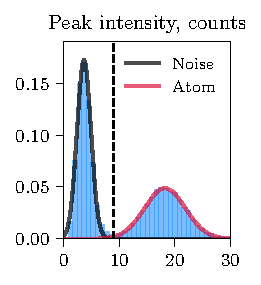
\includegraphics{fig-py/imaging-hist.pdf}
    \hfill
    \addletter{125}{b}
    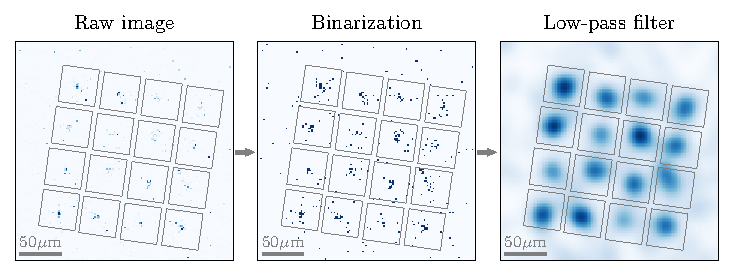
\includegraphics{fig-py/imaging-base.pdf}
    \caption{
        \textbf{Single-atom identification and image processing.}
        a) Histogram of peak intensities extracted from binarized and low-pass filtered images shows a bimodal distribution: the first peak corresponds to camera noise (black), the second corresponds to single atoms (red). The dashed line indicates the threshold used for atom identification.
        b) Image processing pipeline: Raw fluorescence image (left), binarization by intensity thresholding (center), and application of a low-pass filter (right) to reveal spatially localized atomic signals. 
        % \red{Для (a) можно добавить fit, показав что иногда случаются и два атома.}
    }
    \label{fig:imaging-base}
\end{figure}
